\documentclass{scrartcl}
\usepackage[utf8x]{inputenc}
\usepackage[frenchb]{babel}
\usepackage{amssymb}
\usepackage{lmodern}
\usepackage[T1]{fontenc}
\usepackage{verbatim}
\usepackage{ucs}
\usepackage{graphicx}
\usepackage{amsmath}
\usepackage{tikz}
\usetikzlibrary{automata}
\usetikzlibrary {positioning}
\usepackage{multicol}
\usepackage[french, onelanguage, boxed]{algorithm2e}
\SetKwInput{KwOut}{Sorties}
\usepackage{hyperref}

\usepackage{titling}
\usepackage{fancyhdr}
\pagestyle{fancy}
\renewcommand{\headrulewidth}{1pt}
\renewcommand{\footrulewidth}{\headrulewidth}

\newcommand{\brokencell}[2][c]{\begin{tabular}[#1]{@{}c@{}}#2\end{tabular}}
\newcommand{\todo}{\Huge TODO \normalsize}
\usepackage{listings}
\lstset{frame=single, breaklines=true,
          breakatwhitespace=true, basicstyle=\scriptsize,
          showstringspaces=false, escapeinside={(*}{*)},
          keywordstyle=\color{deepblue},
          stringstyle=\color{deepred},
          commentstyle=\color{deepgreen},
          literate=
                   {é}{{\'e}}1{É}{{\'E}}1
                   {è}{{\`e}}1{È}{{\`E}}1
                   {ê}{{\^e}}1{Ê}{{\^E}}1
                   {à}{{\`a}}1{À}{{\`A}}1
                   {ù}{{\`u}}1{Ù}{{\`U}}1
                   {û}{{\^u}}1{Û}{{\^U}}1
                   {ô}{{\^o}}1{Ô}{{\^O}}1
                   {ó}{{\'o}}1{Ó}{{\'O}}1
                   {ç}{{\c c}}1{Ç}{{\c C}}1
                   {œ}{{\oe}}1{Œ}{{\OE}}1
                   {î}{{\^i}}1{Î}{{\^I}}1
        }

\title{Rapport final}
\author{Maxence Ahlouche \and Maxime Arthaud \and Korantin Auguste
  \and Martin Carton \and Thomas Forgione \and Thomas Wagner}
\date{20 décembre 2013}

\begin{document}

  \begin{titlepage}
  \begin{center}
    
\includegraphics[height=1cm]{LogoEnseeiht}\\\vspace{1cm}
    \hrule\vspace{0.5cm}
    \textsc{\Large Graphes et Recherche opérationnelle}
    \\\vspace{0.5cm}

    \textbf{\huge\thetitle}
    \\\vspace{0.4cm}
    \hrule\vspace{2cm}

    \begin{minipage}{0.4\textwidth}
      \begin{flushleft} \large
        \emph{Chef de projet:}\\\hspace{1cm}Martin~\textsc{Carton}
        \emph{Responsable qualité:}\\\hspace{1cm}Maxime~\textsc{Arthaud}
      \end{flushleft}
    \end{minipage}
    \begin{minipage}{0.4\textwidth}
      \begin{flushright} \large
         Maxence~\textsc{Ahlouche}
         Korantin~\textsc{Auguste}
         Thomas~\textsc{Forgione}
         Thomas~\textsc{Wagner}
      \end{flushright}
    \end{minipage}

    \vfill
    {\large 20 décembre 2013}
  \end{center}
\end{titlepage}

  \newpage
  \tableofcontents

  \newpage
  \section{Introduction}
    %Rappel: L'objectif de ce rapport final (CRF6) est de
%         ***corriger les erreurs***
%commises dans les rapports (CRFs) précédents (ndlr: il y en a!) et de
%faire la preuve que les travaux de l'équipe l'ont conduite à
%         ***acquérir des connaissances théoriques***
% dans les divers domaines abordés.

Dans ce rapport, nous allons présenter les différents algorithmes, modèles,
théorèmes, etc.\  que nous avons pu découvrir ou approfondir lors de l'UE de
graphes et recherche opérationnelle. Cette UE était très riche et nous y avons
beaucoup appris. Mais ce rapport ne présentera pas exhaustivement ce que nous
avons fait.

En effet, il ne servira pas à présenter les travaux accomplis lors des
différentes unités d'acquisitions, ni à présenter nos programmes et les
résultats de nos tests (pour cela, se référer aux rapports respectifs des
différentes UAs), mais à présenter les connaissances théoriques que nous avons
acquises.

Il se terminera par un bilan de ce que nous avons acquis lors des différentes
UAs, accompagné de remarques sur notre travail en groupe.


  \newpage
  \section{UA: Graphes}
    % Si vous vous demandez à quoi servent les empty \mbox après les paragraphes,
% vous êtes des boulays, apprenez latex.
\subsection{Introduction}
  La théorie des graphes est un domaine entre les mathématiques et
  l'informatique très utilisé dans la résolution de nombreux problèmes~: cela
  peut aller du routage sur internet au calcul d'itinéraire par des GPS\dots
  
  Nous verrons dans cette section quelques applications des graphes. Une
  dernière application sera vu dans la section~\ref{sec:laby}.

\subsection{Définitions}
  \begin{description}
    \item[Graphe] Un graphe est constitué d'un ensemble de sommets, et d'un
      ensemble d'arêtes (c'est-à-dire des couples de sommets) qui relient ces
      sommets.
      \begin{center}
        \begin{tikzpicture}[node distance=1.5cm,auto]
          \node[draw, circle] (1) at (0,0) {1};
          \node[draw, circle] (2) at (2,-0.5) {2};
          \node[draw, circle] (3) at (4,0) {3};
          \node[draw, circle] (4) at (1,1) {4};
          \node[draw, circle] (5) at (4,2) {5};
          \node[draw, circle] (6) at (0,1.5) {6};

          \path (2) edge node {} (1);
          \path (4) edge node {} (2);
          \path (4) edge node {} (3);
          \path (1) edge node {} (4);
          \path (4) edge node {} (5);
        \end{tikzpicture}
      \end{center}
    \item[Graphe connexe] Un graphe est dit connexe quand on peut aller de
      n'importe quel sommet vers n'importe quel autre sommet en suivant des
      arêtes.
      \begin{center}
        \begin{tikzpicture}[node distance=1.5cm,auto]
          \node[draw, circle] (1) at (0,0) {1};
          \node[draw, circle] (2) at (2,-0.5) {2};
          \node[draw, circle] (3) at (4,0) {3};
          \node[draw, circle] (4) at (1,1) {4};
          \node[draw, circle] (5) at (4,2) {5};
          \node[draw, circle] (6) at (0,1.5) {6};

          \path (2) edge node {} (1);
          \path (4) edge node {} (2);
          \path (4) edge node {} (3);
          \path (1) edge node {} (4);
          \path (4) edge node {} (5);
          \path (4) edge node {} (6);
        \end{tikzpicture}
      \end{center}
    \item[Graphe orienté] Un graphe orienté n'est pas constitué d'arêtes mais
      d'arcs (des paires de sommets).
      \begin{center}
        \begin{tikzpicture}[->, >=stealth', shorten >=1pt, node
          distance=1.5cm,auto]
          \node[draw, circle] (1) at (0,0) {1};
          \node[draw, circle] (2) at (2,-0.5) {2};
          \node[draw, circle] (3) at (4,0) {3};
          \node[draw, circle] (4) at (1,1) {4};
          \node[draw, circle] (5) at (4,2) {5};
          \node[draw, circle] (6) at (0,1.5) {6};

          \draw[arrows={-triangle 90}] (2) --++ (1);
          \draw[arrows={-triangle 90}] (4) --++ (2);
          \draw[arrows={-triangle 90}] (4) --++ (3);
          \draw[arrows={-triangle 90}] (1) --++ (4);
          \draw[arrows={triangle 90-triangle 90}] (4) --++ (5);
        \end{tikzpicture}
      \end{center}
    \item[Graphe complet] Un graphe est dit complet quand tout ses sommets sont
      reliés deux à deux par une arrête. Le nombre de d'arêtes d'un tel graphe
      est alors $\frac {n(n-1)} 2$.
      \begin{center}
        \begin{tikzpicture}[node distance=1.5cm,auto]
          \foreach \x in {0, 72, ..., 359}
            \node[draw, circle] (\x) at (\x:2) {};

          \foreach \x in {0, 72, ..., 359}
            \foreach \y in {0, 72, ..., 359}
              \path (\x) edge node {} (\y);
        \end{tikzpicture}
      \end{center}
    \item[Degré d'un sommet] Le degré d'un sommet est le nombre d'arêtes
      incidentes à ce sommet.
  \end{description}

\subsection{Modélisation mathématique}
Il existe plusieurs moyens de représenter des graphes. Parmi ceux-ci,
le plus simple est la matrice d'adjacence, où l'on stocke une matrice
de taille $n\times n$ ($n$ étant le nombre de sommets), dont chaque
colonne et chaque rangée représente un sommet. La case $i, j$ de la
matrice contient un $1$ si les sommets $i$ et $j$ sont reliés par une
arête (ou un arc dans le bon sens, dans le cas orienté). Évidemment,
cette représentation est loin d'être efficace, la mémoire utilisée
étant exponentielle quand le nombre de sommets du graphe
augmente. Toutefois, elle peut servir pour certains
algorithmes. Notamment, un algorithme de recherche de chemin peut
multiplier la matrice d'adjacence par elle-même $m$ fois~: alors, il
existera un chemin de taille $m$ entre deux sommets si la case
correspondante contient un $1$.
  On notera toutefois que les matrices d'adjacences étant souvent creuses
  (remplies de 0), il existe des moyens de les représenter autrement que
  par un tableau.

  On peut également représenter les graphes par une liste de sommets,
  chacun ayant une liste d'arêtes.
  En mémoire, cette structure est donc constituée d'une liste de pointeurs
  vers des sommets. Les sommets contenant une liste de pointeurs vers des
  arêtes. Chaque arête dispose d'un pointeur vers chaque sommet extrémité.
  Cette structure est évidemment plus efficace, car elle ne stocke que
  les informations nécessaires.


\subsection{Graphes eulériens}
  \subsubsection{Analyse mathématique}
    Un graphe eulérien est un graphe contenant un cycle eulérien, c'est-à-dire
    une chaine parcourant toutes les arêtes du graphe une et une seule fois, en
    revenant au sommet de départ.

    \begin{description}
      \item[Théorème d'Euler] Un graphe connexe est eulérien si et seulement si
        chacun de ses sommets est de degré pair.
    \end{description}

    Un graphe semi-eulérien, quant à lui, contient une chaine eulérienne:
    celle-ci passe également par toutes les arêtes du graphe une seule et
    unique fois, mais ne retourne pas au sommet de départ. Le théorème précédent
    se généralise alors aux graphes semi-eulériens: un graphe connexe est
    semi-eulérien si et seulement tous ses sommets sauf deux sont associés à un
    nombre pair d'arêtes. Dans ce cas, la chaine eulérienne aura pour départ
    l'un des deux sommets associés à un nombre impair d'arêtes et pour sommet
    d'arrivée le deuxième.

  \subsubsection{Méthode de résolution}
    Afin de trouver une chaine ou un cycle eulérien dans un graphe, on peut
    utiliser deux méthodes: une méthode qui teste toutes les possibilités, et
    une autre plus intelligente et moins couteuse.

    \paragraph{Matrices latines}
      La première méthode (voir algorithme~\ref{alg:meth_mat_lat}) est inspirée
      des matrices latines. Chaque coefficient de la matrice sera un ensemble
      de chaines, une chaine étant elle-même une liste de sommets. La matrice
      latine de notre graphe sera la matrice $M$ dont chaque coefficient
      $m_{i,j}$ vaudra:
      \begin{itemize}
        \item l'ensemble vide si le nœud $i$ n'est pas relié au nœud $j$ dans
          le graphe;
        \item un ensemble contenant pour unique élément la chaine  $[N_i,N_j]$
          si les nœuds $i$ et $j$ sont reliés (où $N_k$ représente le nœud
          $k$).
      \end{itemize}

      Nous définissons ensuite un produit sur les coefficients d'une telle
      matrice (voir algorithmes~\ref{alg:prod_mat} et~\ref{alg:prod_chaine}). Le
      produit de deux chaines sera:
      \begin{itemize}
        \item nul si le dernier nœud de la première chaine n'est pas le premier
          nœud du deuxième;
        \item la concaténation des deux chaines sinon.
      \end{itemize}

      Le produit de deux ensembles de chaines sera l'ensemble contenant les
      produits de chaque couple de nœuds.

      Pour tout $k$ entier naturel, le coefficient $(i,j)$ de la matrice $M^k$
      représentera l'ensemble des chaines de longueur $k$ reliant les nœuds $i$
      et $j$.

      Puisque une chaine eulérienne passe une unique fois par chaque arête, il
      suffira de calculer la matrice latine élevée à cette puissance pour
      trouver sur sa diagonale l'ensemble des cycles possibles. En éliminant à
      chaque produit les chaines qui passent plusieurs fois par la même arête,
      on trouve l'ensemble des cycles eulériens.

      La complexité de cet algorithme est exponentielle: calculer la puissance
      de la matrice latine revient en fait à calculer chaque chaine possible dans
      le graphe, et tester si elle est un cycle eulérien ou non.

    \paragraph{Algorithme d'Euler}
      La deuxième méthode, basée sur l'algorithme d'Euler est nettement plus
      efficace. Une fonction récursive cherche un cycle eulérien d'un
      sous-graphe de notre graphe de départ, puis s'appelle récursivement sur
      chacun des sommets parcourus par cette chaine, dans le graphe où l'on a
      supprimé les arêtes déjà parcourues. En reconstruisant ces cycles
      astucieusement, on parvient à trouver un cycle eulérien de complexité
      linéaire en le nombre d'arêtes du graphe.

    \begin{algorithm}
      \KwIn{un graphe}
      \KwOut{%
        la liste des cycles ou chaines eulériens si le graphe est eulérien
        semi-eulérien ou la liste vide sinon
      }
      \Begin{%
        \tcc{Construction de la matrice latine du graphe}
        construire une matrice à n lignes et n colonnes\;
        remplir la matrice de listes vides\;
        \For{chaque nœud du graphe}{%
          \For{chaque arête sortant de ce nœud}{%
            ajouter la liste [noeud de départ, noeud d'arrivée] à la case de
            la matrice correspondante\;
          }
        }
        n $\leftarrow$ le nombre d'arêtes total du graphe\;
        calculer la puissance $(n-1)$ième de la matrice

        \For{chaque coefficient de la matrice ainsi calculée}{%
          \If{le coefficient n'est pas nul}{%
            concaténer ce coefficient à la variable de retour\;
          }
        }
      }
      \caption{Méthode de la matrice latine}
      \label{alg:meth_mat_lat}
    \end{algorithm}

    \begin{algorithm}
      \KwIn{$A$ et $B$ deux matrices latines}
      \KwOut{le produit de ces deux matrices}
      \Begin{%
        construire la matrice de retour à n lignes et n colonnes\;
        initialiser chaque coefficient de cette matrice à la liste vide\;

        \For{chaque coefficient de la matrice de retour}{%
          \For{$k$ allant de $1$ jusqu'à $n$}{%
            calculer les chaines produits entre a(i,k) et b(k,j)\;
            ajouter au coefficient de la matrice ces chaines\;
          }
        }
      }
      \caption{Produit matriciel}
      \label{alg:prod_mat}
    \end{algorithm}

    \begin{algorithm}
      \KwIn{liste\_1 et liste\_2 deux listes de chaine}
      \KwOut{une liste de chaines}
      \Begin{%
        créer une liste de chaine vide (liste de retour)\;
        \For{$i$ dans liste\_1}{%
          \For{$j$ dans liste\_2}{%
            construire la chaine résultante de la concaténation de $i$ et $j$
            (en enlevant le nœud présent deux fois)\;
            construire un ensemble de chaine vide\;
            \For{$k$ allant de $1$ à la longueur de la chaine construit}{%
              construire la chaine élémentaire menant du nœud $k$ au nœud $k+1$\;
              \If{cette chaine n'est pas dans l'ensemble}{%
                ajouter cette chaine dans l'ensemble\;
              }
              \Else{%
                rendre la chaine nulle\;
                sortir de la boucle\;
              }
            }
          }
          \Si{le chaine n'est pas nulle}{%
            concaténer la chaine trouvée à la liste de retour
          }
        }
      }
      \caption{Produit entre listes de chaines (coefficients de matrices
      latines)}
      \label{alg:prod_chaine}
    \end{algorithm}

\subsection{Graphes hamiltoniens}
  \subsubsection{Analyse mathématique}
    Un graphe hamiltonien (resp.\ semi-hamiltonien) est un graphe sur lequel on
    peut trouver un cycle (resp.\ une chaine) passant par tout les sommets une
    et une seule fois. Ce problème est donc celui d'un enfant qui souhaiterait
    visiter de manière unique toutes les salles d'un musée.

    Le problème de savoir si un graphe est (semi-)hamiltonien est NP-complet,
    de même que de trouver un cycle ou une chaine s'il y en a.

    Il existe cependant des conditions suffisantes pour lesquelles on peut
    affirmer qu'un graphe est hamiltonien.

    \begin{description}
      \item[Théorème] Un graphe complet est hamiltonien. C'est une conséquence
        du théorème de Dirac.
      \item[Théorème de Dirac] Un graphe simple à $n$ sommets ($n \ge 3$) dont
        chaque sommet est au moins de degré $\frac{n}{2}$ est hamiltonien.
      \item[Théorème de Ore] Un graphe simple à $n$ sommets ($n \ge 3$) tel que
        la somme des degrés de toute paire de sommets non adjacents vaut au
        moins $n$ est hamiltonien.
      \item[Théorème de Pósa] Un graphe simple à $n$ sommets ($n \ge 3$) est
        hamiltonien si:
        \begin{itemize}
          \item pour tout entier $k$ tel que $1 \le k < \frac{n-1}{2}$ le
            nombre de sommets de degré inférieur ou égal à $k$ est inférieur à
            $k$;
          \item le nombre de sommets de degré inférieur ou égal à
            $\frac{n-1}{2}$ est inférieur ou égal à $\frac{n-1}{2}$.
        \end{itemize}
      \item[Fermeture d'un graphe] La fermeture d'un graphe est le graphe
        construit à partir de celui en rajoutant des arrêtes entre chaque
        sommets $a$ et $b$ tel que $\deg(a)+\deg(b) > n$ tant qu'il en existe.
      \item[Théorème de Bondy et Chvátal] Un graphe est hamiltonien si et
        seulement si sa fermeture est hamiltonienne.

        Ce théorème n'est utile que si l'on peut utiliser l'un des théorèmes
        précédents sur la fermeture.
    \end{description}

  \subsubsection{Méthode de résolution}
    Pour tester si un graphe est hamiltonien on peut utiliser les théorèmes
    précédents. Si le graphe ne respecte les conditions d'aucun de ces
    théorèmes, on recherche une chaine hamiltonienne dans ce graphe.

    Pour rechercher une chaine hamiltonienne dans un graphe, on pourrait
    chercher parmi toutes les chaines possibles. La complexité d'un tel
    algorithme (voir algoritme~\ref{alg:hamil}) dans le pire des cas est donc
    très mauvaise: $O(n!)$. Comme on peut s'arrêter dès qu'on a trouvé une
    chaine sans devoir tester toutes les autres chaines possibles, la
    complexité moyenne sera inférieure.

    \begin{algorithm}
      \KwIn{un graphe}
      \KwIn{un sommet de départ optionnel node\_from}
      \KwIn{un ensemble (éventuellement vide) de nœuds déjà parcouru
      nodes\_done}
      \KwOut{une chaine hamiltonienne sous la forme d'une liste ordonnée de
      sommets, ou None s'il n'en existe pas}

      \Begin{%
        \If{node\_from n'a pas été fourni}{%
          node\_from $\leftarrow$ un nœud du graphe\;
        }
        ajouter node\_from à nodes\_dones\;

        \If{cardinal(node\_from) == ordre(graphe)}{%
          \Return{[node\_from]}
        }

        \For{chaque arête dans le graphe}{%
          autre $\leftarrow$ le sommet opposé à node\_from par rapport à cette
          arête\;
          \If{autre dans nodes\_done}{%
            passer à la prochaine arête
          }
          appeler la fonction récursivement avec le graphe, node\_from et
          nodes\_dones comme paramètres\;
          \If{la liste retournée est non-vide}{%
              y ajouter node\_from au début et la retourner\;
          }
        }
      }
      \caption{Recherche de chaine hamiltonienne}
      \label{alg:hamil}
    \end{algorithm}

\subsection{Problème du postier chinois}
  \subsubsection{Analyse mathématique}
    Le problème du postier chinois consiste à trouver la chaine la plus courte
    dans un graphe connexe non-orienté passant au moins une fois par chaque
    arête, et revenant à son point de départ.

    Ce problème est donc celui du facteur qui souhaite réaliser une tournée
    la plus rapidement possible en passant par toutes les rues et retournant
    à la poste.

    Ce problème peut être réduit à la recherche d'un couplage parfait de cout
    minimum, que peut être résolu en temps polynomial dans le cas général.

    \begin{description}
      \item[Couplage] Un couplage d'un graphe est un ensemble d'arêtes de ce
        graphe qui n'ont pas de sommets en commun.
      \item[Couplage Parfait] Un couplage parfait est un couplage tel que tout
        sommet du graphe est présent une fois et une seule dans le couplage.
      \item[Clique] Une clique est un ensemble de sommets deux à deux
        adjacents.
    \end{description}

  \subsubsection{Méthode de résolution}
    On remarque que dans le cas d'un graphe eulérien, il suffit d'appliquer
    l'algorithme d'Euler (voir algorithmes~\ref{alg:euler}
    et~\ref{alg:couplage} pour avoir la chaine voulue.

    Dans les autres cas, la méthode de résolution consiste à transformer le
    graphe en graphe eulérien, en ajoutant des arêtes. Une méthode possible
    est la suivante:
    \begin{enumerate}
      \item on crée d'abord le graphe partiel contenant uniquement les sommets
        de degré impair;
      \item on transforme ensuite ce graphe en clique: pour chaque couple de
        sommets non reliés entre eux, on crée une arête les rejoignant,
        de poids égal au cout le plus faible possible pour rejoindre ces
        sommets dans le graphe initial (ceci se calcule facilement avec
        l'algorithme de Dijkstra);
      \item on cherche le couplage parfait de cout minimum en utilisant des
        algorithmes comme celui d'Edmonds. On peut aussi tester simplement
        toutes les possibilités;
      \item pour chaque arête de cet ensemble, on double la chaine la plus
        courte reliant les sommets reliés par cette arête dans le graphe initial;
      \item on obtient alors un graphe eulérien, sur lequel on applique
        l'algorithme d'Euler.
    \end{enumerate}

    \begin{algorithm}
      \KwIn{Un graphe non-orienté et connexe g}
      \KwOut{le cycle le plus court permettant de visiter toutes les arêtes de
      g}

      \Begin{%
        \tcc{Création du graphe partiel}
        \For{chaque sommet de g}{%
          \If{le sommet est de degré impair}{%
            créer le sommet dans graphe\_partiel\;
          }
        }
        \For{chaque arête de g}{%
          \If{ses 2 sommets sont dans graphe\_partiel}{%
            créer la même arête dans graphe\_partiel\;
          }
        }

        \tcc{Transformation en clique}
        \For{chaque couple de sommet (s1, s2) dans graphe\_partiel}{%
          \If{il n'y a pas d'arête reliant s1 et s2}{%
            $(cout, chaine) = dijkstra(s1, s2)$\;
            créer l'arête reliant s1 et s2 dans graphe\_partiel, de cout cout\;
          }
        }

        $couplage, cout = aux(ensemble vide, ensemble vide, 0)$\;

        \For{chaque arête dans couplage}{%
          $(s1, s2) =$ sommets reliés par arête dans g\;
          $(cout, chaine) = dijkstra(s1, s2)$\;
          \For{chaque arête dans chaine}{%
            doubler cette arête dans g\;
          }
        }

        \Return{le cycle eulérien de g}
      }
      \label{alg:euler}
      \caption{TODO: trouver un titre}
    \end{algorithm}

    \begin{algorithm}
      \KwIn{arêtes, sommets\_visités, cout}
      \Begin{%
        \If{sommets\_visites contient tous les sommets de graphe\_partiel}{%
          \Return{(arêtes, cout)}
        }
        \Else{%
          $meilleur\_couplage = Vide$\;
          $meilleur\_cout = 0$\;
          \For{chaque arête de graphe\_partiel}{%
            \If{les 2 sommets de l'arête ne sont pas dans sommets\_visites}{%
              arêtes\_copie = copie de arêtes\;
              sommets\_visites\_copie = copie de sommets\_visites\;

              ajouter arête dans arêtes\_copie\;
              couplage, cout = aux(arêtes\_copie, sommets\_visites\_copie, cout +
              cout de arête)\;

              \If{meilleur\_couplage = Vide ou meilleur\_cout > cout}{%
                meilleur\_couplage = couplage\;
                meilleur\_cout = cout\;
              }
            }
          }
          \Return{(meilleur\_couplage, meilleur\_cout)}
        }
      }
      \label{alg:couplage}
      \caption{Recherche du couplage parfait de cout minimum par bruteforce}
    \end{algorithm}

\subsection{Problème du voyageur de commerce}\label{sec:tsp}
  \subsubsection{Analyse mathématique}
    Le problème du voyageur de commerce consiste à chercher un chemin passant
    par tous les sommets du graphe, de longueur minimale.
    Ce problème peut s'illustrer par l'exemple d'une
    fraiseuse qui doit percer des trous dans une plaque le plus
    rapidement possible, ou encore par un car de touristes qui souhaiterait
    trouver l'itinéraire le plus rapide pour visiter un certain nombre de lieux.

    On peut modéliser ce problème par un graphe complet, dont les arêtes ont un
    cout qui correspond à la distance entre chaque sommet, on cherche alors le
    cycle hamiltonien de cout minimal. On sait qu'un tel cycle existe car le
    graphe est complet.

    Cependant trouver un tel cycle est un problème NP-complet~: il n'existe
    donc pas d'algorithme efficace pour trouver ce cycle, à part une recherche
    exhaustive.
    En effet, la seule méthode exacte consisterait à tester toutes les chaines
    hamiltoniennes, et à prendre celle la plus courte, mais le nombre de chaines
    hamiltonniennes croît exponentiellement en fonction du nombre de sommets
    dans le graphe.

    Nous allons donc nous concentrer sur les méthodes approchées de résolution,
    qui peuvent donner de très bons résultats tout en étant rapides.
    Toutefois, le résultat n'est donc pas forcément le plus court.

  \subsubsection{Heuristiques}
    Les heuristiques vont nous permettre de construire un chemin court (par
    rapport au plus court possible), de manière rapide, avec le moins de calcul
    possible.  Étant donné qu'on est confronté à énormément de possibilités
    pendant la recherche, elles vont permettre d'orienter cette dernière, en
    faisant des choix les plus judicieux possibles sur les possibilités à
    explorer.

    \paragraph{Exemple} Une heuristique simple consiste à partir d'un sommet au
    hasard du graphe et d'aller au sommet le plus proche sur lequel on n'est
    pas encore passé (puis à retourner au sommet de départ pour boucler le
    cycle). Cet algorithme est en $O(n)$ et donc rapide. Mais il n'offre
    cependant aucune garantie de résultat, il existe même des graphes pour
    lesquels il donne le pire cycle.

    Plus généralement, chercher parmi les $p$ sommets les plus proches s'avère
    être une solution relativement efficace, avec une complexité en $O(p^n)$
    (donc toujours exponentielle si $p \neq 1$).

    Une méthode purement basée sur cette heuristique consisterait donc à parcourir
    tout le graphe, en allant sur le voisin le plus proche du sommet courant~:

    \begin{algorithm}
      \KwIn{un graphe complet g}
      \KwOut{(cout, cycle) où cycle est un cycle hamiltonien construit selon la
      méthode du plus proche voisin et cout son cout associé sous forme de
      liste de sommets}
      \Begin{%
        cout = 0\;
        cycle = une liste composée d'un sommet de g au hasard\;

        \While{il reste des sommets}{%
          \tcc{On ajoute au cycle le sommet suivant}
          plus\_proche = sommet de g sur lequel on est pas encore passé le
          plus proche du dernier sommet du cycle\;

          cout += cout de plus\_proche au dernier sommet du cycle construit\;
          ajouter plus\_proche au cycle\;
        }

        \tcc{On ferme le cycle}
        cout += cout du dernier au premier sommet de cycle\;
        ajouter le premier sommet de la chaine à cycle\;

        \Return{(cout, cycle)}
      }
      \label{alg:voisin}
      \caption{Plus proche voisin}
    \end{algorithm}

  \subsubsection{Recherche locale}
    Les heuristiques nous donnant des solutions acceptables, choisies avec un
    minimum de «~bon sens~», il est ensuite possible de tenter d'améliorer
    ces solutions, via de la recherche locale.
    Partant d'une solution fournie, on va explorer les solutions voisines
    à cette dernière, afin de voire si on pourrait pas trouver des solutions
    encore meilleures parmi leur voisinage.

    \paragraph{Exemple} Un algorithme de recherche locale adapté au problème
    du voyageur de commerce est le 2-opt (voir algorithme~\ref{alg:2opt}).
    Le principe du 2-opt consiste à tenter d'éliminer les «~boucles~» qui
    pourraient survenir dans le chemin, afin de le rendre plus court.
    \cite{two_opt}

    Ainsi, partant du chemin suivant (qu'on obtiendrait logiquement en suivant
    l'heuristique consistant à aller sur le sommet le plus près):

    \begin{center}
    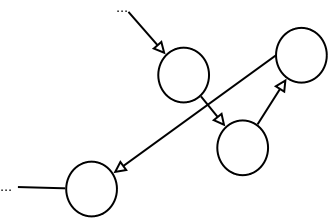
\includegraphics[width=0.3\textwidth]{graphes/2opt1.png}
    \end{center}

    On obtiendrait ceci, en éliminant le croisement:

    \begin{center}
    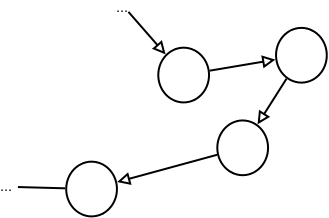
\includegraphics[width=0.3\textwidth]{graphes/2opt2.png}
    \end{center}

    \begin{algorithm}
      \KwIn{un cycle hamiltonien (liste de sommets) et son cout}
      \KwOut{un cycle hamiltonien et son cout inférieur ou égal au coup
      d'entrée}

      \Begin{%
        \For{chaque couple de sommets (a, b) dans le cycle}{%
           $\begin{aligned}
             \text{nouveau\_cout} & \leftarrow
            \text{cout}\\
            &- \text{cout de a à son successeur dans le cycle}\\
            &- \text{cout de b à son successeur dans le cycle}\\
            &+ \text{cout de a à b}\\
            &+ \text{cout du successeur de a au successeur de b dans le
            cycle}\\
          \end{aligned}$\;

          \If{nouveau\_cout < cout}{%
            cout = nouveau\_cout
            cycle = cycle crée en échangeant a et b dans cycle\;
          }
        }
        \Return{(cout, cycle)}
      }
      \caption{2-opt}
      \label{alg:2opt}
    \end{algorithm}

    Il a donc une complexité quadratique du nombre de sommets du cycles.

    L'application du 2-opt sur le chemin obtenu via une heuristique simple peut
    donner des résultats plus proches de la solution optimale qu'on pourrait le
    penser, et la combinaison des deux est donc une bonne méthode.

  \subsubsection{Métaheuristiques}

  Plutôt que d'utiliser une simple heuristique pour trouver une solution à priori plutôt
  bonne, puis d'y appliquer une recherche locale pour tenter de l'améliorer encore,
  il est possible d'utiliser des «~métaheuristiques~».
  Ces algorithmes vont avoir besoin d'heuristiques et de recherche locale, mais vont
  s'en servir en boucle, pour tenter sans cesse de trouver une solution meilleure.

  Ils vont partir explorer différentes parties de l'espace, souvent en guidant
  leur exploration grâce à l'heuristique, et en essayant de retomber sur des
  parties de l'espace les plus intéressantes possibles grâce aux algorithmes de
  recherche locale.

  Il existe énormément de métaheuristiques. En voici quelques uns:
  \begin{description}
  \item[Recherche locale itérée] métaheuristique très simple consistant à
    utiliser une heuristique puis appliquer de la recherche locale pour
    améliorer son résultat.  Ensuite, on perturbe légèrement ce résultat, on
    applique à nouveau une recherche locale et on recommence.
  \item[Recherche tabou] amélioration de la recherche locale itérée, qui va
    utiliser une «~liste taboue~» bannissant toute recherche autour des zones de
    l'espace déjà explorées.
  \item[Recuit simulé] explore d'abord l'espace sans se restreindre aux parties
    donnant des solutions efficaces, puis se restreint de plus en plus au
    voisinage de celles-ci. Converge donc vers les solutions les plus efficaces
    trouvées, puis relâche les contraintes et explore autour de ces dernières,
    quitte à trouver des solutions vraiment moins efficaces. Recommence à se
    contraindre aux plus efficaces, etc\dots
  \item[Algorithmes génétiques] imitent la sélection naturelle, avec une
    population de solutions qui évoluent en mutant et en s'échangeant leurs
    caractéristiques entre elles. On peut même faire évoluer des populations
    séparément avec les modèles en îles, pour avoir plusieurs populations très
    différentes.
  \item[Colonies de fourmis] imitent là encore la nature en simulant des
    phéromones déposées par des fourmis virtuelles, qui orientent la recherche
    au fil du temps.
  \end{description}

  \subsubsection{Conclusion}
    Il est intéressant de constater que les heuristiques, les méthodes de
    recherche locales et les métaheuristiques sont des choses extrêmement
    générales, utilisées pour résoudre énormément de problèmes demandant
    d'explorer un espace extrêmement grand.

    Elles ne sont donc pas propres au voyageur du commerce, même si on a vu
    comment, dans ce cas précis, on pouvait obtenir des résultats corrects en
    se passant de métaheuristiques. On pourrait donc améliorer ces résultats en
    en utilisant.


  \newpage
  \section{UA: Programmation linéaire}
    \subsection{Introduction}
  La programmation linéaire, ou optimisation linéaire, consiste à maximiser (ou,
  de manière équivalente, minimiser) une fonction linéaire sur un polyèdre
  convexe (dont un cas particulier courant est la maximisation sous des 
  contraintes linéaires).

\subsection{Problème du sac à dos}
  \subsubsection{Présentation du problème}
    \begin{center}
\includegraphics[width=120pt]{sac_a_dos.jpg}\end{center}

    Ce problème parait simple en apparence: nous avons un ensemble d'objets,
    chaque objet pouvant avoir une masse différente et ayant une certaine
    valeur, et nous voulons remplir un sac à dos de manière à maximiser la
    valeur totale, sans dépasser une certaine masse maximale.

    Résoudre ce genre de problèmes est utile par exemple en gestion de
    portefeuilles pour trouver le meilleur rapport entre rendement et risque,
    ou en découpe de matériaux, pour minimiser les chutes.

    \paragraph{}
    Ce problème est un problème d'optimisation linéaire. En effet, cela revient
    à résoudre le problème:
    \[ \begin{array}{r|l}
        \displaystyle\max_{i \in S' \subset S} v_i &
        \displaystyle\sum_{i \in S'} m_i \leq W
      \end{array}
    \]
    où $S$ est l'ensemble des objets, $S'$ est un ensemble de $n$ objets
    choisis, $v_i$ la valeur de l'objet $i \in S$, $m_i$ sa masse et $W$ la
    masse maximale autorisée dans le sac.

    Cependant la résolution de ce problème n'est pas simple: déterminer s'il
    est possible de dépasser une valeur minimale sans dépasser le poids maximal
    est un problème NP\nobreakdash-complet.

  \subsubsection{Résolution exacte}
    Une exploration exhaustive de l'ensemble des parties de $S$ n'est pas très
    réaliste, car celui-ci est de cardinal $2^{\mathrm{card} S}$.

    Mais, ce problème peut être résolu en utilisant la programmation
    dynamique\footnote{Qui consiste à résoudre un problème de taille $n$ à
    partir de la résolution d'un problème de taille $n-1$.}. En effet, on peut
    déterminer si un objet $i$ fait partie de l'ensemble des objets à choisir en
    considérant le problème sur l'ensemble $S\backslash\{i\}$ et la masse
    maximale $W-m_i$.
    
    Toutefois, un tel algorithme (voir algorithme~\ref{alg:sacados}) fonctionne
    uniquement si les poids des objets
    sont des entiers. De plus sa complexité en temps est en $O(nW)$ et celle en
    mémoire en $O(W)$\footnote{En pratique on pourrait l'utiliser sur des
    masses non-entières en les multipliant, ce qui augmenterait la complexité
    du même facteur. De plus on peut réduire la complexité temporelle en
    $O(nW')$ avec $W' = \frac W {\mathrm{ppcm}(\text{toutes les masses})}$.}.

  \subsubsection{Résolution approchée}
    Un autre algorithme pour résoudre ce problème, dit algorithme glouton,
    consiste simplement à choisir les «~meilleurs~» objets jusqu'à que la masse
    maximale soit dépassée. Le critère déterminant quels sont les meilleurs
    objets pourrait être la masse faible, le prix élevé, ou le rapport
    prix/masse élevé.

    Cet algorithme est beaucoup plus rapide que le précédent (il a une
    complexité en temps de $O(n \log n)$, pour le tri des objets) et ne
    nécessite en mémoire que la liste des objets. De plus il peut être utilisé
    quand les masses ne sont pas entières. Mais ce n'est qu'un algorithme
    approché qui ne fournit aucune garantie de résultat.


    \paragraph{}
    Un autre algorithme pour résoudre ce problème est inspiré du comportement
    des fourmis: une ``fourmi'' se promène plus ou moins au hasard dans
    l'ensemble des possibilités en marquant les objets choisis comme
    intéressants (comme les fourmis le font avec les phéromones). Ces fourmis
    vont essayer de choisir de plus en plus souvent les objets ayant souvent
    été marqués intéressants. On s'arrête après un certain nombre de tours, ou
    quand les nouvelles itérations ne sont plus considérées suffisamment
    intéressantes.

  \subsubsection{Relation avec le voyageur de commerce}
    Il est intéressant ici de faire le lien avec le problème du voyageur
    du commerce: les solutions utilisées ici sont \emph{les mêmes}.

    En effet, on a vu que ce problème (avec des poids non entiers, donc impossible
    à résoudre par programmation dynamique) se résout seulement par une recherche
    exhaustive.
    
    On a aussi vu comment le résoudre de manière approchée via une heuristique
    simple, et l'algorithme des fourmis est une métaheuristique qu'on a mentionnée
    précédemment.


    Plus intéressant encore, on peut même construire une «~bijection~» entre un
    problème du sac à dos
    et un problème du voyageur de commerce sur un graphe\cite{knapsack_to_tsp}!
    Ceci démontre que ces deux algorithmes sont équivalents, et appartiennent donc à la même
    classe d'algorithmes. % c'est bôoooo les maths :D

\subsection{Problème d'optimisation linéaire}
  Le but du problème est de maximiser une fonction linéaire sous certaines
  contraintes, linéaires elles aussi.

  \subsubsection{Point de vue mathématique}
      Considérons le problème suivant :
      $$ (P) \quad \max_{x\in C \subset \mathbb{R}^n} f(x)$$
      Nous nous placerons dans le cas où $f$ est linéaire, où $x \geqslant 0$,
      et où $C$ est décrit par des contraintes d'inégalités linéaires,
      c'est-à-dire qu'il existe une matrice $A$ et un vecteur $b$ tels
      que $Ax\leqslant b$.

    \paragraph{Existence de solutions}
      Pour un tel problème, trois possibilités s'offrent à nous:
      \begin{itemize}
        \item les contraintes sont incompatibles;
        \item la fonction est non majorée sur $C$;
        \item le problème admet un maximum sur $C$.
      \end{itemize}
      Nous savons de plus que $C$ est un polyèdre convexe. Un théorème garantit
      alors que si ce problème a une solution, alors il s'agit d'un de
      ses sommets. Nous allons donc chercher les solutions parmi les sommets de
      $C$.

  \subsubsection{Algorithme du simplexe}
    Le principe de cet algorithme est de considérer un des sommets du polyèdre,
    puis de se déplacer en suivant les arêtes de ce polyèdre en augmentant à
    chaque itération le gain. L'algorithme se terminera lorsque nous nous 
    trouverons sur un sommet, dont tous les sommets adjacents présentent un gain
    plus faible. La convexité du polyèdre nous garantit que le résultat est 
    optimal.

    L'algorithme du simplexe (algorithme~\ref{alg:simpl}) a une complexité dans
    le pire des cas exponentielle, mais en pratique, cet algorithme est
    efficace.
    
    Cet algorithme ne permet pas de maximiser une fonction pour des variables
    entières (par exemple pour connaitre un nombre de produits à produire, donc
    un nombre entier) à produire pour maximiser un gain (bien qu'on pourrait en
    pratique l'utiliser en considérant que la solution optimale entière est
    suffisamment proche de la solution optimale réelle).

    \paragraph{Forme standard et tableau canonique}
      Pour résoudre le problème, la première étape est le mettre sous forme
      standard. Pour cela on ajoute à chaque inéquation $j$ de la forme
      $\sum a_{j,i}x_i \leq 0$ une variable dite d'écart pour la transformer en
      égalité: $\sum a_{j,i}x_i + s_j = 0$ où $s_j \geq 0$.
      
      Les inéquations de la forme $\sum a_ix_i \geq 0$ sont d'abord multipliées
      par $-1$ avant cette étape.
      %todo: et les égalités on en fait quoi ? J'ai essayé en les transformant
      %en deux inégalités <= et >= mais ça marche pas.

      On construit ensuite un tableau dit canonique représentant le problème
      comme suit:
      \begin{itemize}
        \item la première ligne de la matrice est
          $[m_0, m_1, \cdots, m_n, 0, \cdots, 0]$ où les $(m_i)$ sont les
          coefficients du problème $\min \sum m_ix_i$ et à laquelle on ajoute
          autant de $0$ qu'on a ajouté de variables d'écart;
        \item les autres lignes de la matrice sont
          $[a_{j,0}, \cdots, a_{j,n}, 0, \cdots, 0, 1,0, \cdots, 0]$ où les $1$
          sont placés de manière à former une matrice identité (ils
          correspondent aux variables d'écart ajoutées).
      \end{itemize}

    \paragraph{Exemple}
      Considérons le problème suivant: nous pouvons créer 4 produits à partir
      de 3 ressources. Chaque produit rapporte un certain bénéfice et nous
      cherchons à maximiser notre gain.  
      \begin{center}
        \begin{tabular}{|c|cccc|c|}\hline
          & $P_1$ & $P_2$ & $P_3$ & $P_4$ & stock \\ \hline
          $R_A$ & 2 & 4 & 5 & 7 & 72 \\
          $R_B$ & 1 & 1 & 2 & 2 & 17 \\
          $R_C$ & 1 & 2 & 3 & 3 & 24 \\ \hline
          bénéfice & 7 & 9 & 18 & 17 &  \\ \hline
        \end{tabular}
      \end{center}

      La première étape de l'algorithme revient à constuire le tableau suivant,
      en rajoutant les variables d'écart $x_1$, $x_2$ et $x_3$.

      \begin{center}
        \begin{tabular}{|c|ccccccc|c|}\hline
          & $P_1$ & $P_2$ & $P_3$ & $P_4$ & $x_1$ & $x_2$ & $x_3$ & stock \\ \hline
          $R_A$ & 2 & 4 & 5 & 7 & 1 & 0 & 0 & 72 \\
          $R_B$ & 1 & 1 & 2 & 2 & 0 & 1 & 0 & 17 \\
          $R_C$ & 1 & 2 & 3 & 3 & 0 & 0 & 1 & 24 \\ \hline
          bénéfice & 7 & 9 & 18 & 17 & 0 & 0 & 0 & \\ \hline
        \end{tabular}
      \end{center}

      Le produit qui rapport le plus est $P_3$, et on peut en produire au
      maximum 8 (c'est $\underset{i}{\text{argmin}}
      \frac{\text{stock}(i)}{P_3(i)}$). On va donc en produire le plus
      possible, puis mettre à jour le tableau pour aboutir au tableau suivant:

      \begin{center}
        \begin{tabular}{|c|ccccccc|c|}\hline
          & $P_1$ & $P_2$ & $P_3$ & $P_4$ & $x_1$ & $x_2$ & $x_3$ & stock \\ \hline
          $R_A$ & 1/3 & 2/3 & 0 & 2 & 1 & 0 & -5/3 & 2 \\
          $R_B$ & 1/3 & -1/3 & 0 & 0 & 0 & 1 & -2/3 & 1 \\
          $R_C$ & 1/3 & 2/3 & 1 & 1 & 0 & 0 & 1/3 & 8 \\ \hline
          bénéfice & 1 & -3 & 0 & -1 & 0 & 0 & -6 & -144 \\ \hline
        \end{tabular}
      \end{center}

      Dans la case en bas à gauche se trouve l'opposé du gain. Si on
      recommence, on va donc produire $P_1$ (on en produira $1/3$). Le prochain
      tableau sera donc le suivant:

      \begin{center}
        \begin{tabular}{|c|ccccccc|c|}\hline
          & $P_1$ & $P_2$ & $P_3$ & $P_4$ & $x_1$ & $x_2$ & $x_3$ & stock \\ \hline
          $R_A$ & 0 & 1 & 0 & 2 & 1 & -1 & -1 & 1 \\
          $R_B$ & 1 & -1 & 0 & 0 & 0 & 3 & -2 & 3 \\
          $R_C$ & 0 & 1 & 1 & 1 & 0 & -1 & 1 & 7 \\ \hline
          bénéfice & 0 & -2 & 0 & -1 & 0 & -3 & -4 & -147 \\ \hline
        \end{tabular}
      \end{center}

      On voit maintenant que dans la ligne des bénéfices, les coefficients sont
      tous négatifs ou nuls. Ainsi, quelque soit la direction dans laquelle on
      se déplace, on baissera nécessairement notre gain. Nous avons donc
      atteint l'optimum : le gain maximal sera de 147 et il sera atteint en
      produisant 3 produits $P_1$ et 7 produits $P_3$.



    % todo:
    %       contraintes négatives
    %       cas non borné
    \paragraph{Dégénérescence}
      Un problème du simplexe est dit dégénéré si plus de deux contraintes vont
      devoir être nulles en un sommet. Graphiquement, cela veut dire
      qu'au moins 3 droites vont se rencontrer en un sommet du polyèdre.

      Ceci va empêcher l'algorithme du simplexe de progresser entre deux
      itérations: il va simplement changer de base. Le problème étant que sur
      des cas particuliers, il pourra changer de base sans progresser, puis
      boucler à l'infini en faisant un cycle sur des bases qui n'améliorent pas
      la solution.

      Pour éviter cela, on pourrait utiliser des règles d'anti-cyclage, dont la
      règle de Bland, qui consiste à choisir judicieusement les variables qu'on
      fera entrer et sortir de la base, dans le cas où il y aurait plusieurs
      possibilités aussi intéressantes les unes que les autres.



  \newpage
  \section{UA: Jeux}
    \subsection{Introduction}
  Nous nous intéresserons dans cette section de la résolution de différents
  jeux.

\subsection{Shifumi}
    \begin{center}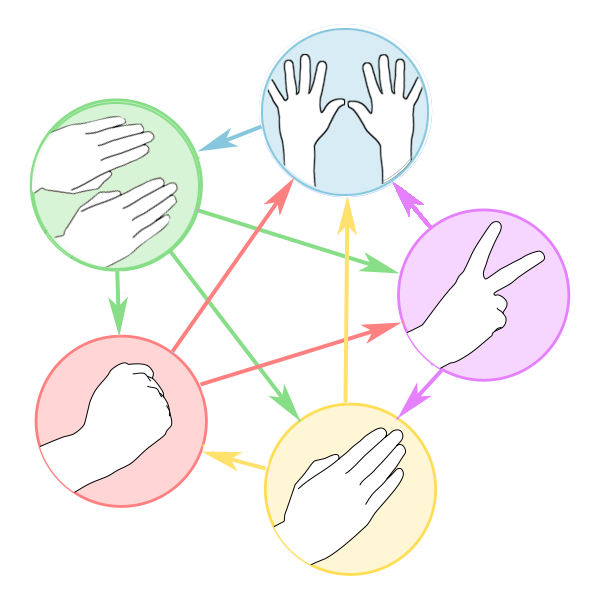
\includegraphics[width=6cm]{shifumi.png}\end{center}

    Une stratégie simple et efficace à laquelle on pourrait penser pour gagner
    au Shifumi serait de jouer de manière aléatoire.

    Et en effet, il s'avère que si les deux joueurs jouent de manière équiprobable,
    on a affaire à un équilibre de Nash~: aucun changement de stratégie de la part
    d'un joueur ne pourra lui permettre d'augmenter ses chances de gagner même
    en connaissant la stratégie adverse.

    De plus, si un adversaire ne joue pas de manière aléatoire (ou augmente la
    probabilité de jouer un certain élément), alors on pourra prévoir ce qu'il
    va jouer et donc trouver une stratégie qui pourra le battre. Les humains
    étant très mauvais pour jouer de manière aléatoire, il est assez facile
    d'écrire une stratégie permettant de les battre.

  \subsubsection{Chaines de Markov}
    Une autre stratégie se base sur des chaines de Markov: en se basant sur les
    derniers éléments joués, elle regarde dans l'historique pour voir l'élément
    qui était joué le plus souvent par l'adversaire après les derniers coups
    joués.

    Cette stratégie s'avère vraiment efficace contre un joueur humain.
    Toutefois, elle est prévisible: si on sait qu'on a affaire à une telle
    stratégie, on peut jouer de manière à la battre.

    C'est pour cela qu'une stratégie aléatoire est la seule pouvant maximiser
    nos gains dans le pire des cas.

  \subsubsection{Variantes}
    Toutes les variantes du Shifumi qui consistent à rajouter des éléments
    pour obtenir un nombre d'éléments pair (par exemple
    pierre/papier/ciseaux/puits) vont créer un déséquilibre, car un élément
    sera moins efficace contre les autres.
    L'équilibre de Nash du jeu va
    alors consister à ne jamais jouer cet élément (et jouer aléatoirement parmi
    les autres).

    Si le nombre d'éléments est impair, alors le jeu pourra être équilibré,
    comme un Shifumi classique.

\subsection{Jeu de la somme magique}
  Ce jeu consiste à choisir, à tour de rôle, $n$ nombres entre 1 et $n^2$ afin
  que leur somme soit égale à $\frac{n(n^2+1)}{2}$.

  \subsubsection{Représentation sous forme de morpion}
Une représentation possible de ce jeu est le carré magique: les
joueurs doivent choisir, l'un après l'autre, une case dans un carré
magique d'ordre $n$, leur but étant de contrôler une ligne, une colonne ou une
diagonale entière de ce carré magique; alors, les nombres qu'ils auront
choisis totaliseront le score voulu. De même, ce problème correspond exactement
au jeu du morpion, étendu à des grilles $n \times n$.

\begin{table}[h]
  \centering
  \begin{tabular}{|cccc|}
    \hline
    16 & 3  & 2  & 13 \\
    5  & 10 & 11 & 8  \\
    9  & 6  & 7  & 12 \\
    4  & 15 & 14 & 1  \\
    \hline
  \end{tabular}
  \caption{Un carré magique d'ordre 4 -- on remarque que les sommes des lignes,
    colonnes et diagonales sont biens égales à $\frac {4(4^2+1)} 2 = 34$}
\end{table}

Ainsi, une des stratégies possibles pour un joueur du jeu de la somme
magique est de construire un carré magique, et de représenter les
nombres choisis par l'adversaire par un rond dans la case
correspondante. Afin de choisir un nombre, il suffit d'appliquer la
stratégie de morpion de son choix sur le carré magique, et de
jouer le nombre correspondant.

Cependant, pour $n>3$, il n'y a pas un seul carré magique d'ordre $n$ (en
ignorant les réflexions et rotations). Cette méthode n'est donc exacte que dans
le cadre des morpions $3\times 3$. En effet, pour de plus grandes tailles les
deux joueurs pourraient jouer dans des carrés magiques différents. D'un point
de vue du morpion, on aura alors l'impression que l'adversaire joue n'importe
quoi, alors qu'il peut être en train de jouer correctement.

\paragraph{}
Le morpion étant un jeu où l'on essaie de minimiser la perte maximum,
on peut s'intéresser à l'algorithme du minimax, pour déterminer une
stratégie non perdante.

\subsubsection{Algorithme du minimax appliqué au jeu du morpion}
L'algorithme du minimax consiste à évaluer toutes les positions de jeu
atteignables depuis la position courante, sur une certaine profondeur
(autrement dit, un certain nombre de tours de jeu), et à jouer de
manière à atteindre la position la plus avantageuse, en supposant que
l'adversaire joue toujours le meilleur coup pour lui-même (ce coup
étant évalué avec notre propre fonction d'évaluation, qui n'est pas
forcément la même que celle de l'adversaire).

Par conséquent, afin d'implémenter l'algorithme du minimax, il faut
commencer par déterminer une fonction d'évaluation.

\paragraph{Fonction d'évaluation}
La fonction d'évaluation que nous avons choisie est très simple: une
ligne, colonne ou diagonale (que nous appelleront désormais simplement
``ligne'') complétée avec notre symbole (ce qui signifie qu'on a
gagné) vaut $+\infty$; si, au contraire, l'adversaire a complété une
ligne, alors cette ligne vaut $-\infty$. Une ligne contenant
uniquement notre symbole rapporte le nombre d'occurrences de notre
symbole dans cette ligne ; à l'inverse, une ligne contenant uniquement
le symbole de l'adversaire rapportera négativement le nombre.
Toutes les autres lignes ne rapportent aucun point.
Ainsi, l'évaluation d'une position de jeu est la somme des points
rapportés par chacune de ses lignes, colonnes et diagonales.

\paragraph{Minimax}
L'algorithme du minimax va construire (implicitement) l'arbre des coups
possibles à partir de la position courante.
L'évaluation d'un nœud de cet arbre sera:
\begin{itemize}
  \item si c'est à notre tour de jouer, le maximum de l'évaluation de nos fils;
  \item si c'est à l'adversaire de jouer, le minimum de l'évaluation
    de ses fils (i.e.\ on suppose que l'adversaire joue le meilleur
    coup à sa disposition, selon la fonction d'évaluation du joueur courant).
\end{itemize}

L'évaluation d'une feuille de l'arbre se fera par la fonction
d'évaluation définie précédemment.

Ainsi, l'algorithme se dirigera naturellement vers la position la plus
avantageuse pour lui.

\subsubsection{Élagage alpha-bêta}
L'élagage alpha-bêta permet de réduire le nombre de nœuds à parcourir durant
l'algorithme du minimax.

Cet algorithme arrête le parcours des fils d'un nœud quand il se rend
compte qu'il ne pourra pas faire mieux.

Dans l'exemple suivant, où les nœuds en bleus sont ceux où l'on doit prendre
le minimum, et ceux en gris le maximum:
\begin{multicols}{2}\begin{center}
  \begin{tikzpicture}[node distance=1.3cm,bend angle=45,auto]
    \node[draw, rectangle, gray] (U) {U};
    \node[draw, circle, blue] (5) [below left=of U] {5};
    \node[draw, circle, blue] (V) [below right=of U] {V};
    \node[draw, rectangle, gray] (4) [below left=of V] {4};
    \node (dots) [below right=of V] {\ldots};

    \path (U) edge node {} (5);
    \path (U) edge node {} (V);
    \path (V) edge node {} (4);
    \path (V) edge node {} (dots);
  \end{tikzpicture}

  Coupure Alpha

  \begin{tikzpicture}[node distance=1.3cm,bend angle=45,auto]
    \node[draw, circle, blue] (U) {U};
    \node[draw, rectangle, gray] (5) [below left=of U] {5};
    \node[draw, rectangle, gray] (V) [below right=of U] {V};
    \node[draw, circle, blue] (4) [below left=of V] {4};
    \node (dots) [below right=of V] {\ldots};

    \path (U) edge node {} (5);
    \path (U) edge node {} (V);
    \path (V) edge node {} (4);
    \path (V) edge node {} (dots);
  \end{tikzpicture}

  Coupure Béta
\end{center}\end{multicols}

On se rend bien compte qu'on n'a pas besoin de parcourir les nœuds suivant,
car on prend le maximum des minimums, ou l'inverse.

Par exemple, pour la coupure alpha: si on trouve des fils de $V$ plus petit
que $4$, on va prendre le maximum, donc c'est $4$ qui sera utilisé, et si on
trouve plus grand ou égal à $5$, on devra prendre le minimum au niveau de $V$,
donc on prendra $5$ dans tous les cas.

Au final, cette amélioration permet de gagner un temps considérable pour
obtenir le même résultat.


\subsection{Duopôles}
  Les jeux précédents sont des jeux non coopératifs à somme nulle (on peut soit
  gagner, soit perdre).

  Il peut aussi être intéressant de voir les jeux à somme non nulle, c'est à
  dire qu'il n'y a pas forcément un gagnant ($1$ point) et un perdant ($-1$
  point), mais il est possible de faire des situations plus ou moins
  gagnant-gagnant, voire même perdant-perdant.

  Le duopôle de Cournot est un bon exemple de ce genre de jeu: il met en jeu
  deux entreprises qui produisent des biens sur le même marché. Elles se font
  donc concurrence, mais plus le marché est inondé de produits, plus leur marge
  est faible (elles peuvent même faire des pertes!).

  \subsubsection{Modélisation}
    On modélise le cout de production unitaire par une constante $\gamma$,
    et le prix de vente unitaire est une fonction affine décroissante de la
    production totale $x+y$ (où $x$ est la production d'une entreprise, et $y$
    celle de l'autre): $p(x, y) = \alpha - \beta\times (x + y)$. Ce dernier est bien
    évidemment commun aux deux entreprises.

    Les gains des entreprises sont donc respectivement:
      \[\begin{array}{c}
        g_1(x, y) = x\times (p(x, y)-c(x)) = x(\alpha+\gamma-\beta(x+y)) \\
        g_2(x, y) = y\times (p(x, y)-c(y)) = y(\alpha+\gamma-\beta(x+y))
      \end{array}\]

    Par la suite, nous noterons $a=\alpha+\sigma$.

  \subsubsection{Stratégies possibles}
    \paragraph{Coopération} Il est possible de coopérer complètement avec
      l'adversaire, en partant du principe que s'il produit autant que nous,
      on maximisera le gain commun de chaque entreprise.
      Cette stratégie permet de très bons gains avec toute autre stratégie qui
      coopère, mais elle se fera souvent écraser par des stratégies qui vont
      «~profiter d'elle~».

      Pour coopérer il suffit de maximiser $g_1(x, y)+g_2(x, y)$ par rapport à
      $x+y$ soit
        \[g_1(x, y) + g_2(x, y) = 2(x+y)(a - \beta(x+y))\]

      Le maximum est donc atteint en $x+y=\frac a {2\beta}$.

      Pour que chaque entreprise ait le même gain, on a $g_1(x, y) = g_2(x, y)$.
      Elles doivent donc produire $x=y=\frac a {4\beta}$.

    \paragraph{Stackelberg}
      % on profite de l'autre, toussa
      TODO

    \paragraph{Œil pour œil, dent pour dent}
      Le principe de cette stratégie est d'être coopérative tant que
      l'adversaire l'est, et de devenir plus agressive quand il ne l'est plus:
      à chaque fois que l'autre joueur n'est pas coopératif, on joue comme le
      ferait la stratégie Stackelberg.

      Une variante de cette stratégie consiste à le pénaliser de plus en plus:
      la première fois on le pénalise une fois, puis deux, puis trois, etc.

      Ces deux stratégies sont efficaces à la fois quand l'autre joueur est
      coopératif (on est alors coopératif) et contre un joueur non-coopératif
      (on devient alors agressif).

\subsection{Conclusion}
  La résolution de jeux est donc un domaine intéressant nécessitant des
  approches très différentes selon le jeu considéré.


  \newpage
  \section{UA: Processus stochastiques}
    \subsection{Introduction}
  La programmation stochastique cherche à étudier la progression au cours du
  temps de processus aléatoires.
  %todo blabla?

\subsection{Théorie des files d'attente}
  Une file d'attente est un système ayant une entrée par laquelle arrivent des
  tâches, ou client, qui attendent leur tour avant d'être traitée une pour en
  sortir.

  Elles sont utilisées pour l'étude de beaucoup de systèmes: attentes de
  clients à des guichets, trafic routier, traitement des tâches par un
  serveur, etc.

  \paragraph{}
  Les files sont étudiées en fonction de la loi qui gère l'entrée, la loi qui
  gère la sortie et le nombre de ``serveurs'' qui traitent les clients.

  La loi de Little est cependant un résultat général:
    \[N = \lambda T_s\]
  où $N$ est le nombre moyen de clients dans le système, $\lambda$ la fréquence
  moyenne d'entrée et $T_s$ le temps moyen passé dans le système.

  \subsubsection{Cas M/M/1}
    On considère une file d'attente où la loi d'entrée suit une loi de Poisson
    de paramètre $\lambda$ ($\lambda$ est dont le nombre moyen d'arrivées par
    unité de temps) et que le temps de service suit une loi exponentielle de
    paramètre $\mu$ ($\frac 1 \mu$ est donc le temps moyen de traitement, sans
    compter l'attente dans la file).

    On dit que ce genre de file d'attente est de type $M/M/1$ selon les
    notations de Kendall.

    Dans ce cas, le nombre moyen d'arrivées pendant le temps de service, appelé
    trafic offert, est $\rho = \frac \lambda \mu$. Le système converge alors si
    et seulement si $\rho < 1$.
    
    \paragraph{}
    La file peut être représentée comme une chaîne de Markov où chaque état $i$
    représente la probabilité qu'il y ait $i$ voitures dans le système (voir
    figure~\ref{fig:markov1}).

    \begin{figure}[h]
      \centering
      \begin{tikzpicture}[->,shorten >=1pt,auto,node distance=2cm,semithick]
        \tikzstyle{every state}=[fill=white,draw=black,text=black,minimum size=1.1cm]

        \node[state] (A) {0};
        \node[state] (B) [right of=A] {$1$};
        \node[state] (C) [right of=B] {$2$};
        \node[state] (D) [right of=C] {$3$};
        \node[minimum size=1cm] (E) [right of=D] {$\cdots$};

        \path (A) edge [bend left] node {$\lambda$} (B);
        \path (B) edge [bend left] node {$\mu$} (A);
        \path (B) edge [bend left] node {$\lambda$} (C);
        \path (C) edge [bend left] node {$\mu$} (B);
        \path (C) edge [bend left] node {$\lambda$} (D);
        \path (D) edge [bend left] node {$\mu$} (C);
        \path (D) edge [bend left] node {$\lambda$} (E);
        \path (E) edge [bend left] node {$\mu$} (D);
      \end{tikzpicture}
      \caption{Représentation d'une file M/M/1 comme une chaine de Markov
        \cite{procstochs_cc}}
      \label{fig:markov1}
    \end{figure}

    Ces états sont liés en régime permanent par les équations:
      \[
        \left\{\begin{aligned}
          \lambda p_0 & = \mu p_1 \\
          \lambda p_1 & = \mu p_2 \\
          & \cdots \\
          \lambda p_n & = \mu p_{n+1} \\
          & \cdots 
        \end{aligned}\right.
      \]
    et
      \[
        \sum_{i=0}^{+\infty} p_n = 1
      \]

    D'où $p_n = \left(\frac \lambda \mu\right)^n p_0 =
     \left(\frac \lambda \mu\right)^n \left(1-\frac \lambda \mu\right) =
     \rho^n (1-\rho)$ (d'où la condition $\rho < 1$).

   Le nombre moyen de clients dans le système est donc:
     \[ N = \sum_{i=0}^n np_n = \frac \rho {1-\rho} \]

   D'après la loi de Little, le temps moyen passé dans le système est donc:
     \[
       T_s = \frac 1 \lambda \frac \rho {1-\rho}
           = \rho \frac \lambda {\mu-\lambda}
     \]

  \subsubsection{Cas M/M/S}
    Une généralisation du cas précédent sont les files de type $M/M/S$, où $S$
    dénote le nombre de serveurs. Les lois d'entrée et sortie restent les mêmes.

    Ces files peuvent aussi être représentées avec les chaînes de Markov (voir
    figure~\ref{fig:markov2}).

    \begin{figure}[h]
      \centering
      \makebox[\textwidth]{\begin{tikzpicture}
        [->,shorten >=1pt,auto,node distance=2cm,semithick]
        \tikzstyle{every state}=[fill=white,draw=black,text=black,minimum size=1.1cm]

        \node[state] (A) {0};
        \node[state] (B) [right of=A] {$1$};
        \node[state] (C) [right of=B] {$2$};
        \node[state] (D) [right of=C] {$3$};
        \node[minimum size=1cm] (E) [right of=D] {$\cdots$};
        \node[state] (F) [right of=E] {$S-1$};
        \node[state] (G) [right of=F] {$\phantom{+}S\phantom{+}$};
        \node[state] (H) [right of=G] {$S+1$};
        \node[minimum size=1cm] (I) [right of=H] {$\cdots$};

        \path (A) edge [bend left] node {$\lambda$} (B);
        \path (B) edge [bend left] node {$\mu$} (A);
        \path (B) edge [bend left] node {$\lambda$} (C);
        \path (C) edge [bend left] node {$2\mu$} (B);
        \path (C) edge [bend left] node {$\lambda$} (D);
        \path (D) edge [bend left] node {$3\mu$} (C);
        \path (D) edge [bend left] node {$\lambda$} (E);
        \path (E) edge [bend left] node {$4\mu$} (D);
        \path (E) edge [bend left] node {$\lambda$} (F);
        \path (F) edge [bend left] node {$(S-1)\mu$} (E);
        \path (F) edge [bend left] node {$\lambda$} (G);
        \path (G) edge [bend left] node {$S\mu$} (F);
        \path (G) edge [bend left] node {$\lambda$} (H);
        \path (H) edge [bend left] node {$S\mu$} (G);
        \path (H) edge [bend left] node {$\lambda$} (I);
        \path (I) edge [bend left] node {$S\mu$} (H);
      \end{tikzpicture}}
      \caption{Représentation d'une file M/M/S comme une chaine de Markov
        \cite{procstochs_cc}}
      \label{fig:markov2}
    \end{figure}

    L'étude de ces chaînes est plus compliquée car les états ne sont plus liés
    par la même équation:
      \[
        \left\{\begin{aligned}
          \lambda p_0 & = \phantom{2\times~}\mu p_1 \\
          \lambda p_1 & = 2\times\mu p_2 \\
          & \cdots \\
          \lambda p_{S-2} & = (S-1)\times\mu p_{S-1} \\
          \lambda p_{S-1} & = S\times\mu p_S \\
          \lambda p_S & = S\times\mu p_{S+1} \\
          \lambda p_{S+1} & = S\times\mu p_{S+2} \\
          & \cdots 
        \end{aligned}\right.
      \]

    On peut montrer que le système est en équilibre si et seulement si
    $\rho = \frac \lambda {S\mu} < 1$. Le nombre moyen de clients et temps
    moyen dans le système sont par contre beaucoup moins intuitifs:
    \[
      \begin{aligned}
        N   &= \rho \left(1 + \frac{P_a}{S-\rho}\right) \\
        T_s &= \frac{1}{\mu} \left(1 + \frac{P_a}{S-\rho}\right)
      \end{aligned}
    \]
    où $\displaystyle P_a = P_0 \frac{\rho^S}{(S-1)!(S-\rho)}$ est la
    probabilité d'attendre et $\displaystyle P_0 = \frac{1}{\sum_{k=0}^{S-1}
    \frac{\rho^k}{k!} + \frac {\rho^S}{S!} \frac {1}{1-\rho/S} }$ est la
    probabilité que le système soit vide.

    On remarque qu'on retrouve bien les mêmes résultats que précédement pour
    $S=1$.



  \newpage
  \section{UA: Ingénierie robotique}
    \subsection{Suivi de murs}
  On s'intéresse ici à la programmation d'un robot\footnote{Un robot en Lego
  Mindstorms NXT, accompagné seulement de deux capteurs à ultrasons et
  deux boutons poussoirs.} afin qu'il puisse longer un mur.

  Afin de longer un mur, on peut par exemple poser un capteur à ultrasons sur
  le côté gauche de notre robot. Lorsqu'il détecte qu'il est trop
  éloigné du mur, il tourne légèrement à gauche. Donc s'il ne détecte plus
  de mur à gauche (le mur tourne) le robot va naturellement tourner à gauche.

  Cette méthode donnant des résultats peu probants si la direction initiale du
  robot n'est pas exactement parallèle au mur, on peut ajouter un autre capteur
  à ultrasons à l'avant du robot. Ainsi, on peut tourner désormais à gauche,
  tout en avançant légèrement, dès qu'on détecte que le mur est trop loin; et
  si on se retrouve face à notre mur, alors on tourne vers la droite jusqu'à ne
  plus l'être.

  Ainsi, on peut suivre un mur droit de manière assez régulière.

\subsection{Labyrinthe}\label{sec:laby}
  \subsubsection{Suivi de mur}
    Pour sortir d'un labyrinthe, le suivi de mur est déjà un algorithme
    admissible, il trouvera une solution s'il en existe une. En effet, si on
    n'arrive pas à sortir du labyrinthe en suivant cette méthode, c'est qu'on 
    longe un ilot dans le labyrinthe, ce qui est impossible si l'on vient
    de l'extérieur.

    L'algorithme de Dijkstra et l'algorithme A* (qui est considéré comme une
    extension du premier) sont utilisés pour trouver le chemin le plus court
    permettant de sortir du labyrinthe.

  \subsubsection{Algorithme de Dijkstra}
    L'algorithme de Dijkstra est un algorithme permettant de trouver le plus
    court chemin entre deux sommets d'un graphe (orienté ou non): il est donc
    utile dans le cas du labyrinthe, car celui-ci peut être représenté comme un
    graphe. En effet il suffit de représenter chaque intersection du labyrinthe
    comme un sommet du graphe, et chaque chemin du labyrinthe par une arête du
    graphe comme sur l'illustration suivante:

    \begin{center}
      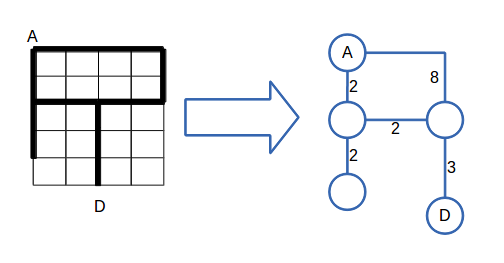
\includegraphics[width=0.55\textwidth]{../slides/jeux/GRO_graph1.png}
    \end{center}

    La complexité de cet algorithme est polynomiale suivant le nombre de sommets
    du graphe.

    Son principe est simple: il parcourt le graphe en gardant en mémoire la
    longueur du chemin le plus court vers chaque sommet.

  \subsubsection{Algorithme A*}
    L'algorithme A* est une amélioration de Dijkstra, qui utilise une heuristique
    pour orienter la recherche.
    Si l'heuristique est bien choisie, il est même possible de s'assurer qu'A*
    donnera bien le résultat optimal (et plus rapidement que Dijkstra).

    Cet algorithme utilise deux listes de nœuds: une liste, dite ouverte, qui
    contient les nœuds explorables et une liste, dite fermée, qui contient les
    nœuds déjà explorés.

    \begin{itemize}
      \item On crée un nœud en lui attribuant un cout heuristique qui
        correspond à la somme du cout du nœud et d'une estimation de la distance de ce
        nœud à l'arrivée.

        Remarque: l'utilisation de ce cout heuristique constitue une différence
        notable avec l'algorithme de Dijkstra, elle permet de s'assurer que
        l'on va toujours plus ou moins dans la bonne direction.

        Par exemple dans un graphe en étoile avec des branches de même taille
        et plusieurs nœuds par branches où l'on part du centre pour rejoindre
        l'extrémité d'une branche l'algorithme de Djkstra explore toutes les
        branches simultanément alors qu'avec l'utilisation du cout heuristique
        on explore directement et uniquement la bonne branche.
      \item On ajoute ce nœud à la liste ouverte.
      \item On prend le nœud qui a le meilleur cout heuristique dans la liste
        ouverte et on l'ajoute à la liste fermée.
      \item On crée les nœuds adjacents et pour chacun d'eux:
        \begin{itemize}
          \item leur cout est égal à la somme des couts de leurs prédécesseurs
            et du cout entre les deux;
          \item si l'un d'eux est présent dans la liste ouverte on vérifie si
            ce nouveau chemin trouvé est plus rapide. Si c'est le cas on
            remplace celui qui est dans la liste ouverte par le nouveau sinon
            on oublie le nouveau;
          \item s'il est déjà dans la liste fermée c'est qu'il a déjà été
            traité ou qu'il est en train d'être traité donc on l'oublie;
          \item et s'il n'est ni dans la liste ouverte ni dans la liste fermée,
            on l'ajoute à la liste ouverte.
        \end{itemize}
    \end{itemize}
	
    À la fin, en remontant tous les prédécesseurs, on remonte le chemin le plus
    court.

  \subsection{Construction du labyrinthe par le robot}
    Cependant pour pouvoir appliquer ces algorithmes il faut connaitre le
    labyrinthe, afin de construire son graphe.

    Or ceci est loin d'être évident: le robot n'ayant aucun moyen de se repérer
    avec précision dans l'espace, il lui faudrait se baser sur la vitesse des
    moteurs pour déterminer sa position. Mais cette méthode peut se révéler
    très mauvaise notamment si le robot change souvent la vitesse d'un moteur
    (pour tourner par exemple) ou s'arrête souvent: il va alors accumuler les
    erreurs de position. De plus, le sol et les roues n'étant pas parfaits, le 
    robot dérape relativement souvent, ce qui augmente encore les erreurs.

  \subsection{Conclusion}
    Le problème du robot dans un labyrinthe est assez simple en théorie. Mais,
    comme souvent, la pratique est bien plus compliquée, car en plus des
    mathématiques qui sont derrière ce problème, viennent des problèmes
    intrinsèques aux robots.

% vim: shiftwidth=2 softtabstop=2 tabstop=2 spell spelllang=fr


  \newpage
  \section{Bilan}
    % Un bilan devra être présenté dans ce dernier rapport final sur la façon de
% travailler de l'équipe au cours de toutes les UAs. Une autoévaluation devra y
% être conduite de sorte à faire apparaitre les points positifs et/ou les
% disfonctionnements apparus dans l'équipe.

\subsection{Enseignement}

% wtf les séances de TD
Nous avons été surpris de la façon dont fonctionnent les séances de
TD, et avons eu du mal à nous y faire: lors des séances, nous étions
censés être lâchés sur les différents problèmes et nous renseigner par
nous-mêmes.  Toutefois, le professeur présent se mettait souvent à
présenter des choses au tableau, et nous ne savions plus trop si nous
devions avancer, ou stopper tout travail et l'écouter. De plus, il
était souvent difficile de savoir si le professeur s'adressait à un
seul groupe ou à toute la classe; enfin, il n'était généralement pas
trivial de discerner la structure des informations données.

% chacun a quasiment rien vu
Il a aussi été assez frustrant de se répartir le travail: comme nous
étions dans un groupe de 6 et avions quand même un certain nombre de
choses à faire, il fallait forcément se concentrer sur un seul
problème. Du coup, chacun a simplement abordé quelques points précis
sur chaque UA, et n'a pas vraiment acquis de connaissances poussées
sur tout le reste des sujets abordés.

% rapports, rapports...
Le fait de devoir faire des rapports à chaque séance était aussi très
lourd à gérer, et assez peu pratique: nous avions l'impression de
passer énormément de temps à écrire des rapports. Ajouté au rapport
final, cela donne un travail de rédaction très important.

\subsection{Travail en groupe} % sujet trollesque :D

% git
L'utilisation d'un gestionnaire de version nous a permis de nous
faciliter énormément le travail en centralisant tout le code et les
rapports.  Pour les rapports de fin de séance, nous avons aussi
utilisé un «~pad~», qui permet d'éditer à plusieurs du texte en temps
réel (alternative libre et simpliste à Google Docs).

Concernant le travail en groupe, il est clair que travailler en groupe
de 6 en faisant en sorte que tout le monde travaille efficacement
n'est pas évident.

Nous avons donc essayé de nous répartir le travail le plus
efficacement possible mais ça n'a pas non plus évident: à de
nombreuses reprises, il fallait se recentrer et essayer de se
re-répartir les tâches clairement, et ce n'est pas évident.  Il y a
donc eu certaines séances très peu productives (ou alors seulement sur
certains points), avec aussi des pertes de motivation lors de certaines
UAs.

Toutefois, les tâches étaient quand même généralement assignées à des
binômes ou trinômes, et le travail a, dans l'ensemble, été plutôt
efficace.

\subsection{Apprentissage}
  Une chose reste certaine: nous avons tous appris de nouvelles choses pendant
  cette UE, même si elles ne reflètent qu'une partie de ce qui était demandé.

  Le fait de se répartir le travail nous a aussi permis de travailler sur ce
  qui nous intéressait le plus, ce qui est plutôt motivant, quand on a
  eu un sujet qui nous intéressait. Malheureusement, nos centres
  d'intérêts étant souvent les mêmes, il n'était pas rare d'être déçu
  par son affectation. Notamment, nous ne nous sommes pas bousculés
  pour travailler sur Sisyphe, avec raison: ce logiciel s'est avéré
  horrible à prendre en main, et le groupe qui a travaillé sur les
  scarabées a pu coder un programme de tests équivalent en autant de
  temps qu'il a fallu à l'autre groupe pour maitriser cet ``outil''.


  \newpage
  \begin{thebibliography}{99}
    \bibitem{bib:proglin:sac_wiki}
  Wikipédia, \emph{Problème du sac à dos},\\
  \url{http://fr.wikipedia.org/wiki/Probl\%C3\%A8me_du_sac_\%C3\%A0_dos}
\bibitem{bib:proglin:en_sac_wiki}
  Wikipedia, \emph{Knapsack problem},\\
  \url{http://en.wikipedia.org/wiki/Knapsack_problem}
\bibitem{bib:proglin:gen}
  David Pisinger's optimization codes,\\
  \url{http://www.diku.dk/~pisinger/codes.html}

  \end{thebibliography}
\end{document}
